\section{Implementation}
\label{sec:implementation}
This section outlines the software resources of our language identification system, explains the necessary data preprocessing steps, and describes the model architecture of our neural networks in more detail.
% TODO: elaborate more, set chapter in context of this thesis

\subsection{Software}
\label{sec:software}

	Our language identification system is implemented in Python~3 and uses the open-source deep learning framework Keras~\cite{chollet2015keras} with the TensorFlow backend~\cite{abadi2016tensorflow} for training our neural networks. Keras provides us with a set of higher-level machine learning primitives (such as convolutional layers) and optimization algorithms (including \emph{stochastic gradient descent}), without sacrificing any fine-grained control over the training parameters. Internally, Keras builds on Google's open-source numerical operation library TensorFlow, which is optimized for quickly computing multidimensional data on GPUs. We make heavy use Keras's aforementioned primitives, especially convolutional layers and the efficient LSTM implementation. Using the TensorFlow framework not only future-proofs our implementation but also enables us to readily deploy our model on mobile phones in the future.

	All models are stored on disk during training, including a summary of the layer architecture as well as the models' weights. This makes it easy to load, evaluate, and deploy all the models later. During the evaluation phase, all performance metrics (accuracy, precision, recall, F1 score) are calculated using the Scikit Learn framework~\cite{scikit-learn}. All measurements are logged and visualized using TensorBoard,\footnote{\url{https://www.tensorflow.org/how_tos/summaries_and_tensorboard/}, accessed 30 January 2017} both for the training and the validation set. Having the ability to easily study and compare different metrics such as accuracy and the loss value across several training runs made it very comfortable to continuously monitor the progress of our research. Figure~\ref{fig:tensorboard} shows a TensorBoard instance with plots of the metrics for several models.
%
	\begin{figure}[tp]
  		\centering
    	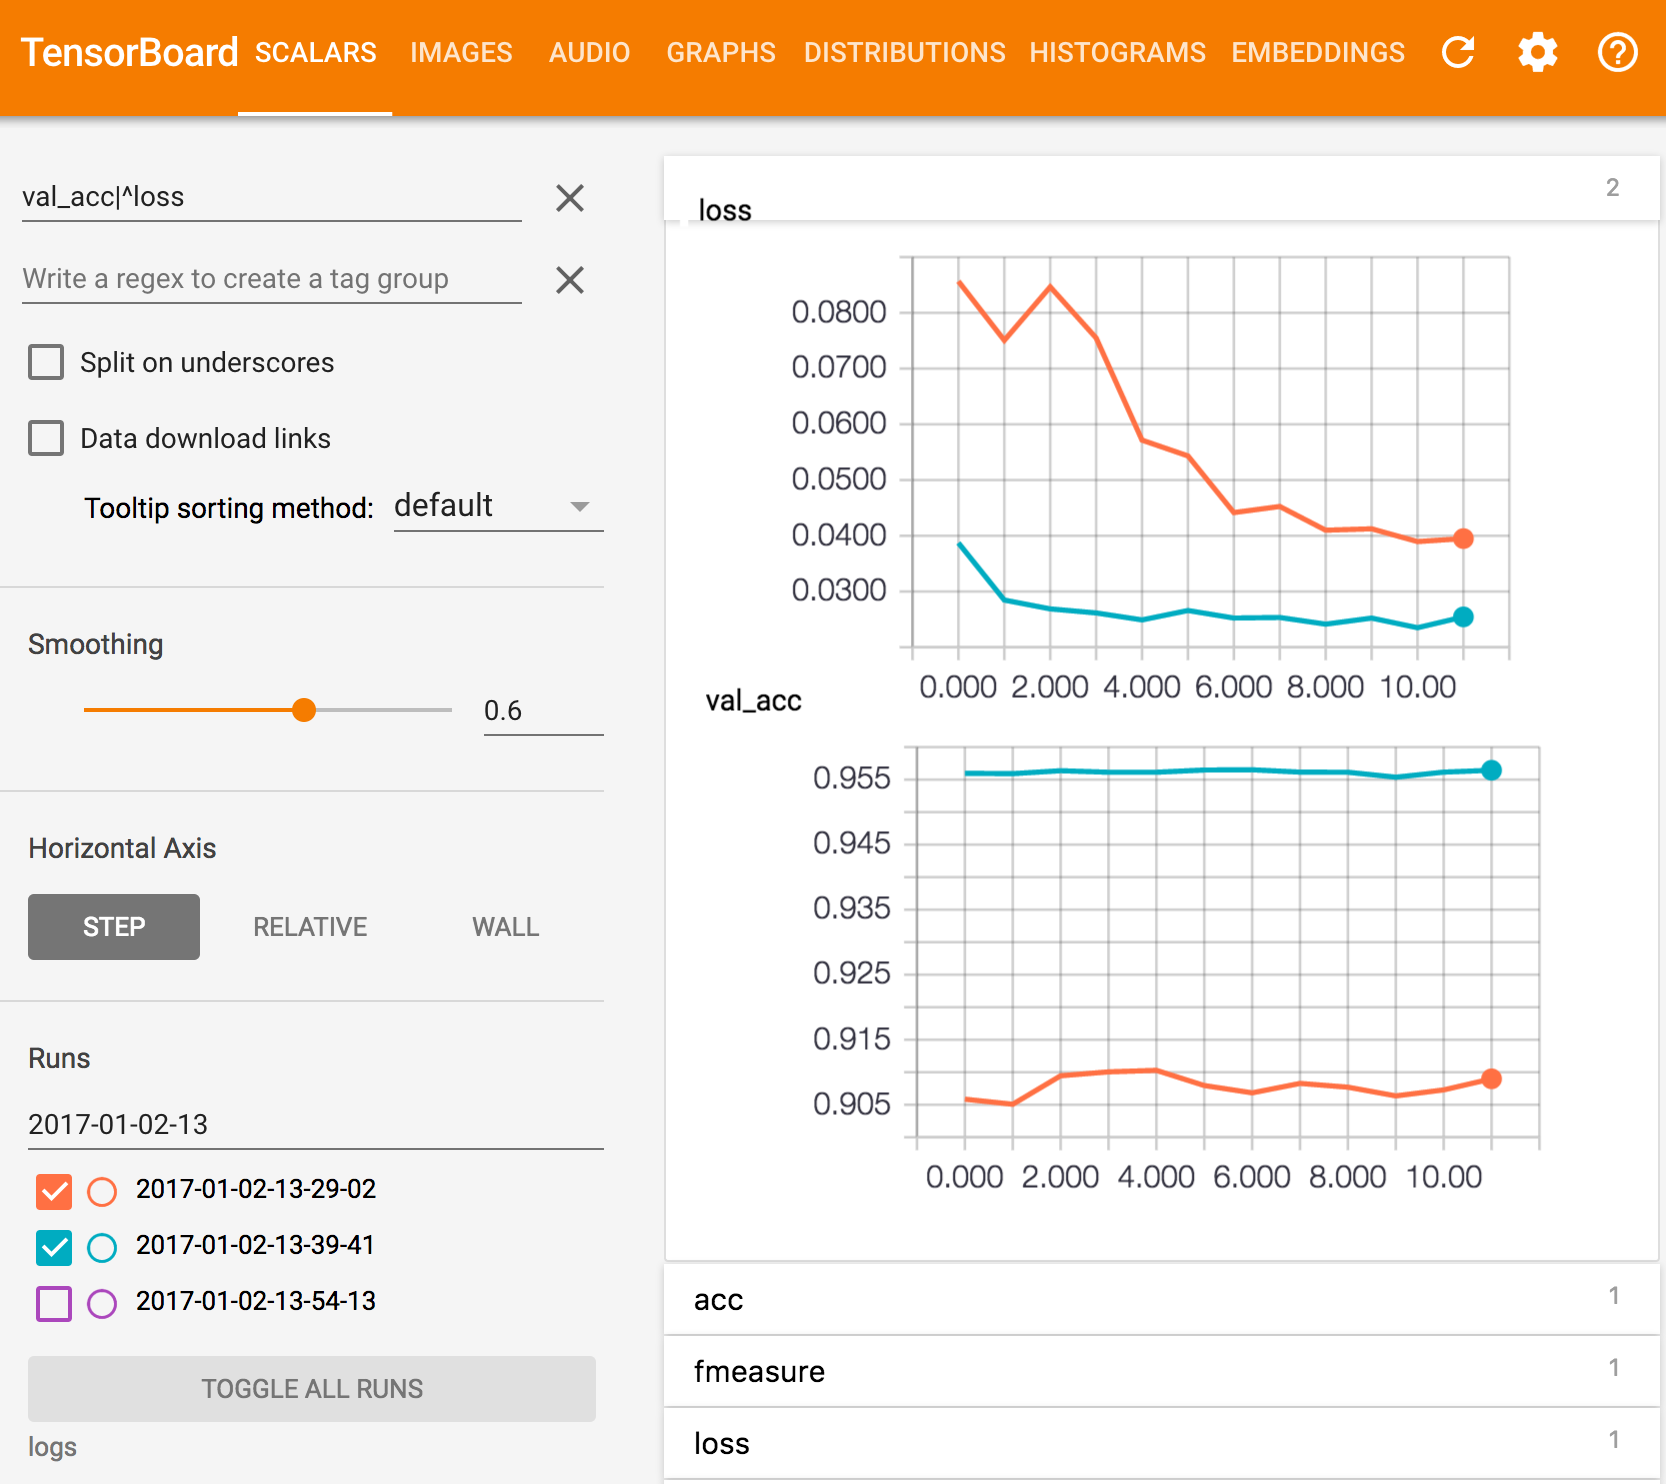
\includegraphics[width=\textwidth,keepaspectratio]{img/tensorboard2.png}
    	\caption{A TensorBoard instance showing training loss and validation accuracy of two different models. We regularly tried different approaches and model architectures and plotted multiple evaluation measures for comparison. This workflow enabled us to judge the impact of each experiment and measure the overall performance progress of the system.}
    	\label{fig:tensorboard}
	\end{figure}
%
We regularly compared different approaches and models against each other and used these plots to select the best performing systems for further experiments.

\subsection{Data Preprocessing}
\label{sec:data_processing}

	All audio files undergo preprocessing before being fed to the neural network. As a first step, all files are encoded in the uncompressed, lossless Waveform Audio File Format (WAVE\footnote{\url{http://www.microsoft.com/whdc/device/audio/multichaud.mspx}, accessed 23 February 2017}), commonly known by its file extension \texttt{*.wav}. This conversion has two advantages. First, a lossless data codec allows for future audio manipulations without any deterioration in signal quality and, second, makes the data easily interchangeable with third-party programs and libraries such as SciPy~\cite{scipy}.

	Since none our neural networks operate on raw waveform audio signals directly, we transfer our features into the image domain. As introduced in Section~\ref{sec:audio_representations}, we use a spectrogram representation of the audio data for training our models. The spectrograms are generated using the open-source command line tool SoX.\footnote{\url{http://sox.sourceforge.net/}, accessed 23 February 2017} The spectrograms are discretized using a Hann window~\cite{blackman1958measurement} and \num{129}~frequency bins along the frequency axis ($y$~axis), as instructed by the SoX manual.\footnote{\url{http://sox.sourceforge.net/sox.pdf}, p.~32, accessed 26 March 2017}

	Male human voice frequencies begin between \SI{150}{\hertz}~and \SI{255}{\hertz}~\cite{traunmuller1993frequency}. Female voice frequencies are usually shifted by one octave and begin at~\SI{210}{\hertz}. Typically, voice frequencies range up to~\SI{3.4}{\kilo\hertz}. For reference, the human ear is capable of recognizing frequencies from \SI{20}{\hertz}~to \SI{20}{\kilo\hertz}, with most sensitivity in the region of between \SI{300}{\hertz}~and \SI{10}{\kilo\hertz}. Single sounds, however, exceed this limit significantly. Generally, voice frequencies are influenced by gender, age, as well as various other factors, such as the language, the type of discourse, and the emotional state of the speaker. Figure~\ref{img:frequencies} shows the frequency areas with high energy in response to the tone of different vowels of human speech for the English language.
%
	\begin{figure}[tp]
  		\centering
    	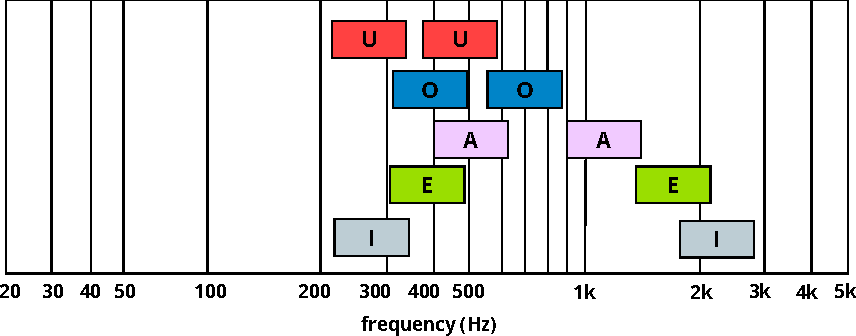
\includegraphics[width=\textwidth,keepaspectratio]{img/frequencies.pdf}
    	\caption{The upper and lower frequency areas (\emph{formant}) for different vowels, typical for human speech. The lower speech formant $F_1$ has a total range of about \SI{300}{\hertz} to \SI{750}{\hertz} and the higher speech formant $F_2$ about \SI{900}{\hertz} up to over \SI{3000}{\hertz}. But each single spoken tone has a much narrower range for both formants.}
    	\label{img:frequencies}
	\end{figure}
%

Most phonemes in the English language do not exceed \SI{3000}{\hertz} in conversational speech.
Consequently, we instructed SoX to only include frequencies of up to~\SI{5}{\kilo\hertz} in the spectrograms.
The time axis ($x$~axis) is rendered at \num{25}~pixels per second. Each audio sequence is clipped into nonoverlapping ten-second segments. To avoid padding issues and segments shorter than ten seconds, the final segment is discarded. Since we gathered enough training data, we decided against padding with black pixels, which could be interpreted as silence and add unnaturally long speech pauses. We also decided against filtering silent sections within the ten-second audio segments to preserve the natural pauses between words and to not disturb the regular speech rhythm. Frequency intensities are mapped to an eight-bit grayscale range. We combined all audio channels into a single mono channel in order to generate only a single spectrogram image. The resulting grayscale images are saved as lossless, $500 \times 129$ PNG files. Listing~\ref{lst:spectrograms} shows the SoX command for generating a spectrogram image from an input audio file.

	\begin{listing}[tp]
	\begin{lstlisting}[caption={SoX command and options used for generating monochrome spectrograms. All audio files were discretized into \num{129}~frequency buckets using a constant pixel width per time step, resulting in spectrogram images of $500 \times 129$ pixels.}, label={lst:spectrograms}]
sox -V0 input.wav -n remix 1 rate 10k spectrogram -y 129 -X 50 -m -r -o spectrogram.png

V0 - verbosity level 
n - apply filter/effect
remix - select audio channels
rate - limit sampling rate to 10k; caps max frequency at 5kHz according to Nyquist-Shannon sampling theorem
y - spectogram height
X - pixels per second for width
m - monochrome output
r - disable legend
o - output file
    \end{lstlisting}
    \end{listing}

	As seen in Figure~\ref{fig:spectrogram}, the spectrograms feature very apparent bright ripple-like patterns.
%
	\begin{figure}[tp]
  		\centering
    	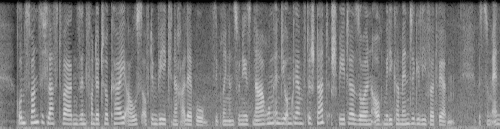
\includegraphics[width=\textwidth,keepaspectratio]{img/spectrogram.png}
    	\caption{A spectrogram generated from a German ten-second audio clip using SoX. Notice the bright ripple-like patterns representing intense frequency activations. We hypothesize that these frequency activations are suitable as the main features for the classifier.}
    	\label{fig:spectrogram}
	\end{figure}
%
	Each of these patterns represents a strong activation of a certain frequency at a point in time. Several frequency activations can be active simultaneously, constituting a particular phoneme or sound. A sequence of these phonemes forms words and is only interrupted by short speech pauses. We hypothesize that our \ac{lid} system learns the characteristical and unique composition of these frequency activations for every language in our classifier.

\subsection{Neural Network Architectures}
\label{sec:cnn_architecture}
To successfully solve our research task with deep neural networks, we have to design a fitting model architecture. Combing the right layers and adjusting the parameters correctly is not a trivial task. Critics argue that deep learning systems are a black box and that the impact of the individual layout of the network layers is hard to understand. Therefore, we base our model architectures on proven existing designs from related work and adapt them to our needs, while heeding best practices~\cite{mishkin2016systematic, szegedy2016rethinking}.

The architecture and the number of parameters of a deep neural network suited for a given task is determined by the bias--variance tradeoff~\cite{geman1992neural}. It is the goal of a network's author to avoid underfitting or overfitting the resulting model. Bias characterizes the prediction error that results from the model's limited ability to learn relevant relations between features in the training data. Underfitting can be caused by designing too small or too few network layers, causing a high bias. Variance, in contrast, refers to the error that results from the model responding overly sensitive to variation in the training data. Designing a too large network, introducing too many parameters, or adding too many layers result in a model with low variance. Hence, the model learns an exact representation of the training data without abstracting for more general applications. This is known as \emph{overfitting}.

Designing and adjusting the network layout is an iterative process. We tried many variations and parameters of our proposed model layouts to find the most suitable design for our LID system. The layout of the network interdepends and interacts with other design decisions of the system, especially the loss calculation. Each change in parameters involves a complete new training run to judge the effect of the change. Hence, the architecture always needs to be tested in its entirety.

In this thesis, we tried three different designs of convolutional neural networks. The first and second ones are based on the early VGGNet-like CNN-M model architectures by Simonyan et al.~\cite{Chatfield14}. The CNN features five convolutional layers and modest feature map output sizes. Note that the network's first two convolutional layers have comparatively large kernel size of $7 \times 7$ pixels and $5 \times 5$ pixels, respectively, yielding a large receptive field. Each convolutional layer is followed by batch normalization~\cite{ioffe2015batch}, a technique that helps in increasing training speed and achieving a higher level of model regularization. Following these layers, we added a $2 \times 2$ pooling layer with a stride of~\num{2}. After the five convolutional layers, we added regularization through a \SI{50}{\percent}~dropout before flattening all parameters to a fully-connected layer with \num{1024}~output units. The final, fully-connected layer serves as a classifier that outputs the language identification predictions. Henceforth, we refer to this model as CNN\_A. The full network layout can be seen in Table~\ref{tab:layers_CNN_A}.
%
 \begin{table}[tp]
  \centering
  \begin{tabu}{rcccc}
  \toprule
\textbf{Layer Type} & \multicolumn{2}{c}{\textbf{Output Size}} & \textbf{Kernel} & \textbf{Stride} \\
                          & \textbf{CNN\_A} & \textbf{CNN\_B} &             &     \\\midrule
Convolution               & 16     & 16   & $7 \times 7$  & 1   \\
Max Pooling               & 16     & 16   & $2 \times 2$  & 2   \\
Convolution               & 32     & 32   & $5 \times 5$  & 1   \\
Max Pooling               & 32     & 32   & $2 \times 2$  & 2   \\
Convolution               & 64     & 32   & $3 \times 3$  & 1   \\
Max Pooling               & 64     & 32   & $2 \times 2$  & 2   \\
Convolution               & 128    & 64   & $3 \times 3$  & 1   \\
Max Pooling               & 128    & 64   & $2 \times 2$  & 2   \\
Convolution               & 256    & 64   & $3 \times 3$  & 1   \\
Max Pooling               & 256    & 64   & $2 \times 2$  & 2   \\
Dropout \& Flatten        & 3328   & 832  &               &     \\
Fully-Connected           & 1024   & 256  &               &     \\
Fully-Connected           & 4      & 4    &               &     \\
  \bottomrule
  \end{tabu}
  \caption{The layerwise architecture for the convolutional neural networks CNN\_A and CNN\_B. These designs are based on early VGG-like networks and features large kernel size for the first two convolutional layers in an effort to capture a large receptive field of features.}
  \label{tab:layers_CNN_A}
 \end{table}

A slightly adapted version of CNN\_A has the same number of convolutional layers but features fewer feature maps. Instead of doubling the initial value of \num{16}~feature maps for every convolutional layer, we stick to a schedule of \num{16}--\num{32}--\num{32}--\num{64}--\num{64} feature maps, respectively. The fully-connected layer is also reduced to only \num{256}~output units. Overall, this model has significantly less parameters than CNN\_A. The purpose of this variation is to ensure that the architecture proposed for CNN\_A is not unnecessarily complex. We called this variation CNN\_B. The network layout of CNN\_B is also listed in Table~\ref{tab:layers_CNN_A}.

Lastly, we evaluate architecture CNN\_C, which is based on the VGGNet-16 network~\cite{simonyan2014very} and uses constant kernel size of $3 \times 3$ for all convolutional layers. At the same time, we increase the number of convolutional layers to seven and extend the number of feature map outputs for each layer to \num{64}--\num{128}--\num{256}--\num{256}--\num{512}--\num{512}--\num{512}. In CNN\_C, all fully-connected layers of are identical to CNN\_A. The main difference of this network design are smaller kernel sizes and, hence, a smaller receptive field of the convolutional layers. To compensate for this, we increase the number of layers. The complete CNN\_C architecture is laid out in Table~\ref{tab:layers_CNN_C}.
%
  \begin{table}[tp]
  \centering
  \begin{tabu}{rccc}
  \toprule
\textbf{Layer Type}              & \textbf{Output Size}  & \textbf{Kernel} & \textbf{Stride} \\ \midrule
Convolution             & 64     & $3 \times 3$    & $1 \times 1$  \\
Max Pooling             & 64     & $2 \times 2$    & $2 \times 2$  \\
Convolution             & 128    & $3 \times 3$    & $1 \times 1$  \\
Max Pooling             & 128    & $2 \times 2$    & $2 \times 2$  \\
Convolution             & 256    & $3 \times 3$    & $1 \times 1$  \\
Convolution             & 256    & $3 \times 3$    & $1 \times 1$  \\
Max Pooling             & 256    & $2 \times 2$    & $2 \times 2$  \\
Convolution             & 512    & $3 \times 3$    & $1 \times 1$  \\
Convolution             & 512    & $3 \times 3$    & $1 \times 1$  \\
Max Pooling             & 512    & $2 \times 2$    & $2 \times 2$  \\
Convolution             & 512    & $3 \times 3$    & $1 \times 1$  \\
Max Pooling             & 512    & $2 \times 2$    & $2 \times 2$  \\
Flatten                 & 6144   &                 &               \\
Fully-Connected         & 1024   &                 &               \\
Fully-Connected         & 4      &                 &               \\
  \bottomrule
  \end{tabu}
  \caption{The layerwise architecture for the convolutional neural network CNN\_C. With seven convolutional layers, this network design is deeper than the other two proposed CNN architectures. Additionally, the number of feature maps is increased to \num{512}~units compared to the \num{256}~units of the CNN\_A network. Overall, this network consists of a higher number of parameters than present in the other two designs.}
  \label{tab:layers_CNN_C}
 \end{table}


For our CRNN hybrid network, we construct a convolutional neural network followed by a recurrent neural network. Specifically, we use a bidirectional \emph{long short-term memory network} (\ac{lstm}) for the RNN part. We decided on using a bidirectional model of two LSTMs instead of a single LSTM based on the successful results of Shi et al.~\cite{shi2016end}. The CNN part of this network is tasked with extracting visual features and providing a high-dimensional intermediate frequency representation. The \ac{rnn} part splits the intermediate interpretation into a series of vectors (along the $x$ axis), which it treats as if they belonged to consecutive time steps.

In the CNN part, we repurpose the CNN\_A network architecture of five convolutional layers with larger kernels for the first two layers, since we found this CNN layout to work best for our LID task (details are provided later in Section~\ref{sec:results_news}). We also keep the batch normalization and max pooling layers. The bidirectional LSTM layer consist of two single LSTMs with \num{256}~output units each. We concatenate both outputs to a vector of \num{512}~dimensions and feed this into a fully-connected layer with \num{1024}~output units serving as the classifier. The complete model architecture can be seen in Table~\ref{tab:layers_CRNN}.
%
 \begin{table}[tp]
  \centering
  \begin{tabu}{rccc}
  \toprule
\textbf{Layer Type}       & \textbf{Output Size}    & \textbf{Kernel} & \textbf{Stride}  \\ \midrule
Convolution               & $123 \times 494 \times 16$  & $7 \times 7$    & $1 \times 1$    \\
Max Pooling               & $61 \times 247 \times 16$   & $2 \times 2$    & $2 \times 2$    \\
Convolution               & $57 \times 243 \times 32$   & $5 \times 5$    & $1 \times 1$    \\
Max Pooling               & $28 \times 121 \times 32$   & $2 \times 2$    & $2 \times 2$    \\
Convolution               & $26 \times 119 \times 64$   & $3 \times 3$    & $1 \times 1$    \\
Max Pooling               & $13 \times 59 \times 64$    & $2 \times 2$    & $2 \times 2$    \\
Convolution               & $11 \times 57 \times 128$   & $3 \times 3$    & $1 \times 1$    \\
Max Pooling               & $5 \times 56 \times 128$    & $2 \times 2$    & $2 \times 1$    \\
Convolution               & $3 \times 54 \times 256$    & $3 \times 3$    & $1 \times 1$    \\
Max Pooling               & $1 \times 53 \times 256$    & $2 \times 2$    & $2 \times 1$    \\
Transpose                 & $53 \times 1 \times 256$    &        &         \\
Reshape                   & $53 \times 256$           &        &         \\
Bidirectional LSTM & 1024                    &        &         \\
Fully-Connected    & 4                       &        &         \\
  \bottomrule
  \end{tabu}
  \caption{The layerwise architecture of the convolutional recurrent neural network. The network consists of two parts, a CNN and a bidirectional LSTM. This design shares its CNN architecture with the previously introduced CNN\_A. The final convolutional layer is sliced into time steps along the $x$ axis (time axis) and serves as input to LSTM.}
  \label{tab:layers_CRNN}
 \end{table}

We decided on training both parts of the hybrid network separately. First, we trained the CNN part by itself. This simplifies the task of learning the frequency features for the network. In practical terms, this means that we could reuse the model weights of the previously trained CNN\_A model. For the RNN part, we used a fine-tuning approach. This means that we froze all convolutional layers' weights by disallowing any further weight updates during the training phase. The bidirectional LSTM and \ac{fc} layers, however, remained unfrozen and continued to be subject to weight updates and were, hence, trained regularly. Later, we also experimented with unfrozen RNN weights, meaning that we trained and updated both the CNN and LSTM layers at the same time. This approach, however, yielded worse results, and we did not pursue it further.
